\documentclass[preview]{standalone}

\usepackage{amsmath}
\usepackage{amssymb}
\usepackage{tikz}
\usepackage{stellar}
\usepackage{definitions}
\usepackage{bettelini}

\begin{document}

\id{geofisica-atmosfera}
\genpage

\section{Atmosfera}

\begin{snippetdefinition}{autora-polare}{Aurora polare}
    L'\textit{aurora polare} è un fenomeno
    caratterizzato visivamente da bande luminose che assumono un'ampia gamma di forme e colori, rapidamente mutevoli nel tempo e nello spazio,
    causato dall'interazione di particelle cariche con la ionosfera (contenente le radiazioni del Sole).
\end{snippetdefinition}

\includesnpt[width=90\%|src=/snippet/static/aurora.avif]{centered-img}

\plain{
    L'aurora boreale si vede solo di notte perché è buio.
Viene denominata <b>aurora boreale</b> qualora si verifichi nell'emisfero nord (boreale),
mentre il nome <b>aurora australe</b> è riferito all'analogo dell'emisfero sud (australe). 
}
\plain{Il criterio per definire lo strato dell'atmosfera è principalmente la temperatura.}

\begin{snippetdefinition}{nebbia}{Nebbia}
    La \textit{nebbia} è un fenomeno dato dalla saturazione di acqua nell'aria,
    come le nuvole, il valore acque satura l'aria e crea un deposito visibile di goccioline.
\end{snippetdefinition}

\begin{snippet}{d9bc89bb-32ae-4742-9a2f-82048d4199d7}
    Quando l'aria è satura di vapore acqueo essa si deposita su oggetti oppure piccole particelle nell'aria.
    \\
    La quantità di vapore acqueo, in grammi, contenuta in un metro cubo d'aria di chiama \textbf{umidità assoluta}.
    L'\textbf{umidità relativa} è il rapporto fra quella assoluta e il valore massimo che può raggiungere.
    \\    
    La condensa che si forma quando apro una finestra è data dal fatto che la temperatura si abbassa, e quindi
    il limite di saturazione si abbassa e l'aria diventa satura.
\end{snippet}

\begin{snippet}{salita-aria-motivi}
    L'aria può salire verso l'alto per tre motivi:
    \begin{enumerate}
        \item perché è calda e umida, e quindi leggera;
        \item perché incontra una montagna che la ostacola;
        \item perché si scontra con una massa d'aria più fredda ed è costretta a salirvi sopra;
        \item perché a terra, si scontra con un'altra massa d'aria ed entrambe vanno verso l'alto.
    \end{enumerate}
\end{snippet}

\begin{snippet}{88ecba26-6d09-4b80-96d3-584a9484ac50}
    Il vento è dato dalle differenze di pressione (come l'acqua nei bicchieri)
    genera spostamenti di masse di aria.
    Questa differenza di pressione è data dalla differenza di temperatura e vapore dell'aria,
    la quale sale o scende creando delle correnti.
    Quando l'aria si muove verso l'alto, la pressione a terra diminuisce,
    mentre quando l'aria fredda scende verso il basso, la pressione a terra aumenta
    (in altitudine si avrebbe l'opposto).
    \\
    All'equatore (dove è più caldo), l'aria sale maggiormente, causando una pressione minore.
    \\
    Il vento non scorre tuttavia dai poli all'equatore a bassa quota e dall'equatore ai poli in alta quota,
    per via della forza di Coriolis.
\end{snippet}

\section{La pressione atmosferica e lo sviluppo dei venti}

\begin{snippetdefinition}{ciclone-definition}{Ciclone}
    L'aria calda si scontra sul suolo e va verso l'alto, creando bassa pressione.
\end{snippetdefinition}

\begin{snippetdefinition}{anticiclone-definition}{Anticiclone}
    L'aria fredda si scontra in aria e va verso il basso, creando alta pressione.
\end{snippetdefinition}

\begin{snippet}{ciclo-aria-cicloni-illustration}
    \begin{figure}[h]
        \centering
        \begin{minipage}{0.37\textwidth}
            \centering
            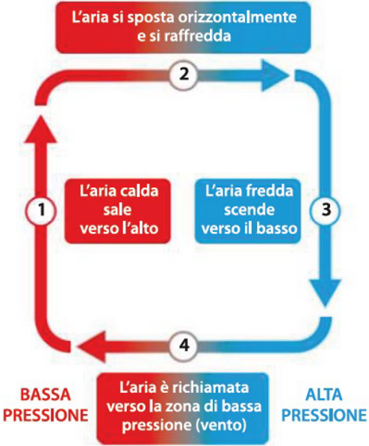
\includegraphics[width=\linewidth]{resources/ciclo-aria.png}
        \end{minipage}\hfill
        \begin{minipage}{0.60\textwidth}
            \centering
            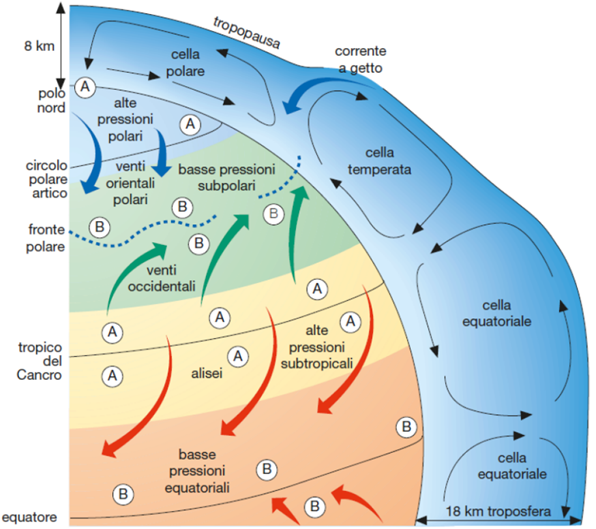
\includegraphics[width=\linewidth]{resources/cicloni.png}
        \end{minipage}
    \end{figure}
    \vspace{0.25cm}
\end{snippet}

\end{document}